\section{Trigonometria}\label{subsec:ss_trigo}

\subsection{Definizioni}

\begin{figure}[H]
\centering
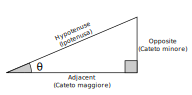
\includegraphics[width=0.7\textwidth]{trigo_01.pdf}
\end{figure}


\begin{equation}
\sin(\theta)=\frac{
\textrm{Opposite}
}{
\textrm{Hypotenuse}
}
\end{equation}

\begin{equation}
\cos(\theta)=\frac{
\textrm{Adjacent}
}{
\textrm{Hypotenuse}
}
\end{equation}

\begin{equation}
\tan(\theta)=\frac{
\textrm{Opposite}
}{
\textrm{Adjacent}
}
\end{equation}

\begin{equation}
\mathrm{cosec }(\theta)=\frac{
1
}{
\sin{\theta}
}
\end{equation}


\begin{equation}
\sec(\theta)=\frac{
1
}{
\cos{\theta}
}
\end{equation}


\begin{equation}
\cot(\theta)=\frac{
1
}{
\tan{\theta}
}
\end{equation}



\setcounter{equation}{0}

\subsection{Formule}

\begin{equation}
\cos^2\theta+\sin^2\theta=1
\end{equation}

\begin{equation}
\tan(\theta)=\frac{\sin(\theta)}{\cos(\theta)}
\end{equation}

\begin{equation}
1+\tan^2\theta=\sec^2\theta
\end{equation}

\begin{equation}
1+\cot^2\theta=\mathrm{cosec }^2\theta
\end{equation}


\begin{equation}
\sin(–\theta) = – \sin(\theta)
\end{equation}

\begin{equation}
\cos(–\theta) = -\cos(\theta)
\end{equation}

\begin{equation}
\sin(x+y)=\sin x \cos y + \cos x \sin y
\end{equation}

\begin{equation}
\sin(x-y)=\sin x \cos y - \cos x \sin y
\end{equation}


\begin{equation}
\cos(x+y)=\cos x \cos y + \sin x \sin y
\end{equation}

\begin{equation}
\cos(x-y)=\cos x \cos y - \sin x \sin y
\end{equation}




\begin{equation}
\tan(x+y)=\frac{
\tan x + \tan y
}{
1- \tan x \tan y
}
\end{equation}



\begin{equation}
\tan(x+y)=\frac{
\tan x - \tan y
}{
1 + \tan x \tan y
}
\end{equation}


\begin{equation}
\sin 2x = 2 \sin x \cos x = \frac{
2\tan x
}{
1+\tan^2x
}
\end{equation}


\begin{equation}
\cos 2x =  \cos^2 x - \sin^2 x = 
1-2\sin^2x=
2\cos^2x-1=
\frac{
1-\tan^2 x
}{
1+\tan^2x
}
\end{equation}


\begin{equation}
\tan 2x=\frac{
2\tan x
}{
1-\tan^2x
}
\end{equation}



\begin{equation}
\sin 3x=3\sin x - 4 \sin^3x
\end{equation}

\begin{equation}
\cos 3x=4\cos^3 x - 3 \cos x
\end{equation}

\begin{equation}
\tan 3x = \frac{
3\tan x - \tan^3x
}{
1-3\tan^2x
}
\end{equation}

\begin{equation}
\sin x \cos y = \frac{1}{2}[ \sin(x+y)+sin(x-y) ]
\end{equation}

\begin{equation}
\cos x + \cos y =2\cos \left(
\frac{x+y}{2}
\right)
\cos \left(
\frac{x-y}{2}
\right)
\end{equation}

\begin{equation}
\cos x - \cos y =-2\sin \left(
\frac{x+y}{2}
\right)
\sin \left(
\frac{x-y}{2}
\right)
\end{equation}


\begin{equation}
\sin x - \sin y =2\cos \left(
\frac{x+y}{2}
\right)
\sin \left(
\frac{x-y}{2}
\right)
\end{equation}

\begin{equation}
\sin x + \sin y =2\sin \left(
\frac{x+y}{2}
\right)
\cos \left(
\frac{x-y}{2}
\right)
\end{equation}

\begin{equation}
\cos\left( \frac{x}{2} \right) = \pm \sqrt{\frac{1+\cos x}{2}}
\end{equation}


\begin{equation}
\sin\left( \frac{x}{2} \right) = \pm \sqrt{\frac{1-\cos x}{2}}
\end{equation}

\setcounter{equation}{0}

\subsection{Triangoli}

\subsubsection{Links}

\href{https://www.math.it/formulario/trigonometria.htm}{math.it}\footnote{\texttt{https://www.math.it/formulario/trigonometria.htm}}
, \href{https://learning.cambridgeinternational.org/classroom/pluginfile.php/155369/mod\_resource/content/4/0580\_Teaching\_Pack\_Understanding\_Bearings\_v2.pdf}{Cambridge International}\footnote{\texttt{https://learning.cambridgeinternational.org/classroom/pluginfile.php/155369/mod\_resource/}

\texttt{content/4/0580\_Teaching\_Pack\_Understanding\_Bearings\_v2.pdf}}


\subsubsection{Teorema di Eulero}\label{subs_euler}

\begin{figure}[H]
\centering
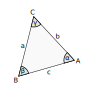
\includegraphics[width=0.3\textwidth]{trigo_04.pdf}
\end{figure}




Anche chiamato il teorema dei seni.

In un triangolo qualunque è costante il rapporto tra la misura di un lato e il seno dell’angolo opposto:


\begin{equation}
\frac{a}{\sin (\alpha)} = \frac{b}{\sin (\beta)} = \frac{c}{\sin (\gamma)}
\end{equation}

\subsubsection{Teorema delle proiezioni}

In un triangolo qualunque la misura di un lato è uguale alla somma dei prodotti delle misure di ciascuno 
degli altri due per il coseno degli angoli che essi formano con il primo:

\begin{equation}
\begin{array}{ll}
a=b\cdot \cos (\gamma) + c\cdot \cos (\beta)  \\
b=a\cdot \cos (\gamma) + c\cdot \cos (\alpha)  \\
c=a\cdot \cos (\beta) + b\cdot \cos (\alpha) 
\end{array}
\end{equation}

\subsubsection{Teorema di Carnot}\label{subs_carnot}

In un triangolo qualsiasi il quadrato di un lato è uguale alla 
somma dei quadrati degli altri due lati diminuita del doppio prodotto 
di questi due lati per il coseno dell’angolo fra essi compreso.

\begin{equation}
\begin{array}{ll}
a^2=b^2+c^2-2\cdot b\cdot c\cos(\alpha)\\
b^2=a^2+c^2-2\cdot a\cdot c\cos(\beta)\\
c^2=a^2+b^2-2\cdot a\cdot b\cos(\gamma)
\end{array}
\end{equation}

Nota: Il teorema di Carnot generalizza il Teorema di Pitagora,
a cui si riduce se si considera un triangolo rettangolo.

\subsubsection{Area di un triangolo}\label{subs_areatgl}

\begin{equation}
\textrm{Area = }\frac{1}{2}ab \sin(\gamma)
\end{equation}

\subsection{Esercizi}

\begin{enumerate} % esercizi

\item 

\begin{figure}[H]
\centering
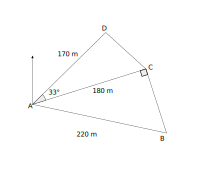
\includegraphics[width=0.7\textwidth]{trigo_02.pdf}
\end{figure}

The diagram shows five straight footpaths in a park.

\begin{itemize}
\item AB=220m
\item AC=180m
\item AD=180m
\item Angle ACB=90$^\circ$
\item Angle DAC=33$^\circ$
\end{itemize}

Calculate BC and CD.

\rightline{( Soluzione a pagina \pageref{stri_01} \label{etri_01}\label{etri_01} )}


\item 

Trovare l'altezza dell'edificio in figura in base ai dati ivi forniti.

\begin{figure}[H]
\centering
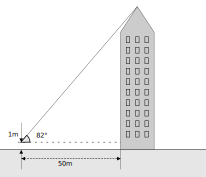
\includegraphics[width=0.7\textwidth]{trigo_05.pdf}
\end{figure}
\rightline{( Soluzione a pagina \pageref{stri_02} \label{etri_02}\label{etri_02} )}


\item 

Dimostrare che 

\begin{equation*}
\frac{
\cos(x)
}{
\tan(x)\cdot\left(1-\sin(x)\right)
} = 1+\frac{1}{\sin(x)}
\end{equation*}
\rightline{( Soluzione a pagina \pageref{stri_03} \label{etri_03}\label{etri_03} )}

\item 

\begin{equation*}
\frac{
1+2\sin(x)\cos(x)
}{
\sin(x)+\cos(x)
}
=
\sin(x)+\cos(x)
\end{equation*}
\rightline{( Soluzione a pagina \pageref{stri_04} \label{etri_04}\label{etri_04} )}

\end{enumerate} % esercizi


